\documentclass{article}\usepackage[]{graphicx}\usepackage[]{color}
%% maxwidth is the original width if it is less than linewidth
%% otherwise use linewidth (to make sure the graphics do not exceed the margin)
\makeatletter
\def\maxwidth{ %
  \ifdim\Gin@nat@width>\linewidth
    \linewidth
  \else
    \Gin@nat@width
  \fi
}
\makeatother

\definecolor{fgcolor}{rgb}{0.345, 0.345, 0.345}
\newcommand{\hlnum}[1]{\textcolor[rgb]{0.686,0.059,0.569}{#1}}%
\newcommand{\hlstr}[1]{\textcolor[rgb]{0.192,0.494,0.8}{#1}}%
\newcommand{\hlcom}[1]{\textcolor[rgb]{0.678,0.584,0.686}{\textit{#1}}}%
\newcommand{\hlopt}[1]{\textcolor[rgb]{0,0,0}{#1}}%
\newcommand{\hlstd}[1]{\textcolor[rgb]{0.345,0.345,0.345}{#1}}%
\newcommand{\hlkwa}[1]{\textcolor[rgb]{0.161,0.373,0.58}{\textbf{#1}}}%
\newcommand{\hlkwb}[1]{\textcolor[rgb]{0.69,0.353,0.396}{#1}}%
\newcommand{\hlkwc}[1]{\textcolor[rgb]{0.333,0.667,0.333}{#1}}%
\newcommand{\hlkwd}[1]{\textcolor[rgb]{0.737,0.353,0.396}{\textbf{#1}}}%

\usepackage{framed}
\makeatletter
\newenvironment{kframe}{%
 \def\at@end@of@kframe{}%
 \ifinner\ifhmode%
  \def\at@end@of@kframe{\end{minipage}}%
  \begin{minipage}{\columnwidth}%
 \fi\fi%
 \def\FrameCommand##1{\hskip\@totalleftmargin \hskip-\fboxsep
 \colorbox{shadecolor}{##1}\hskip-\fboxsep
     % There is no \\@totalrightmargin, so:
     \hskip-\linewidth \hskip-\@totalleftmargin \hskip\columnwidth}%
 \MakeFramed {\advance\hsize-\width
   \@totalleftmargin\z@ \linewidth\hsize
   \@setminipage}}%
 {\par\unskip\endMakeFramed%
 \at@end@of@kframe}
\makeatother

\definecolor{shadecolor}{rgb}{.97, .97, .97}
\definecolor{messagecolor}{rgb}{0, 0, 0}
\definecolor{warningcolor}{rgb}{1, 0, 1}
\definecolor{errorcolor}{rgb}{1, 0, 0}
\newenvironment{knitrout}{}{} % an empty environment to be redefined in TeX

\usepackage{alltt}
\usepackage[sc]{mathpazo}
\usepackage[T1]{fontenc}
\usepackage{geometry}
\usepackage[utf8]{inputenc}
\usepackage{amsmath}
\usepackage{float}
\usepackage{caption}
\usepackage{subcaption}
\usepackage[demo]{graphicx}
\usepackage{booktabs}
\geometry{verbose,tmargin=2.5cm,bmargin=2.5cm,lmargin=2.5cm,rmargin=2.5cm}
\setcounter{secnumdepth}{2}
\setcounter{tocdepth}{2}
\usepackage{url}
\usepackage[unicode=true,pdfusetitle,
 bookmarks=true,bookmarksnumbered=true,bookmarksopen=true,bookmarksopenlevel=2,
 breaklinks=false,pdfborder={0 0 1},backref=false,colorlinks=false]
 {hyperref}
\hypersetup{
 pdfstartview={XYZ null null 1}}
\usepackage{breakurl}
\usepackage{array}
\newcommand\Mark[1]{\textsuperscript#1}
\renewcommand{\hlcom}[1]{\textcolor[rgb]{0.678,0.584,0.686}{\textbf{#1}}}%
\IfFileExists{upquote.sty}{\usepackage{upquote}}{}
\begin{document}



\begingroup
\centering
{\LARGE Predicting Chromatin Conformation From ChIPseq Transcription Factor\\[1.5em]
\large Ricky Lim\Mark{1}, Samuel Collombet\Mark{2}, Nicolas Bertin\Mark{1}, Agus Salim\Mark{3}, Touati Benoukraf\Mark{1}}\\[1em]
\begin{tabular}{*{3}{>{\centering}p{.25\textwidth}}}
    \Mark{1}Cancer Science Institute of Singapore, National University of Singapore&\Mark{2}Institut de Biologie de l', Ecole Normale Superieur de Paris& \Mark{3}Department of Mathematics and Statistics, La Trobe University& \tabularnewline
\url{benoukraf@nus.edu.sg}
\end{tabular}\par
\endgroup

\section{Introduction}

\textbf{The Idea}:
\\ 
\\
ChIPseq could identify not only the direct binding sites of the chromatin protein of interest, but also the indirect ones. 
This owes to the existance of chromatin conformations or complexes. The formation of such complexes will cluster co-factors in close proximity.
\\ 
Here, we are interested in the identification of not only the \textit{direct} binding sites but also the \textit{indirect} ones. With such knowledge, we could predict the chromatin conformation of the protein of interest.
\\

\textbf{Question:} 
\begin{itemize}
    \item Could we cluster the direct and indirect bindings of chromatin proteins from ChIP-seq experiment using Mixture Models (MMs) ?
    \item Could we cluster the direct and indirect bindings of chromatin proteins from ChIP-seq experiment using Mixture Models (MMs), followed by local clusterings (distance proximity) ?
\end{itemize}
    

\newpage
\section{Pipeline Overview}
\begin{figure}[h!] 
    \centering 
    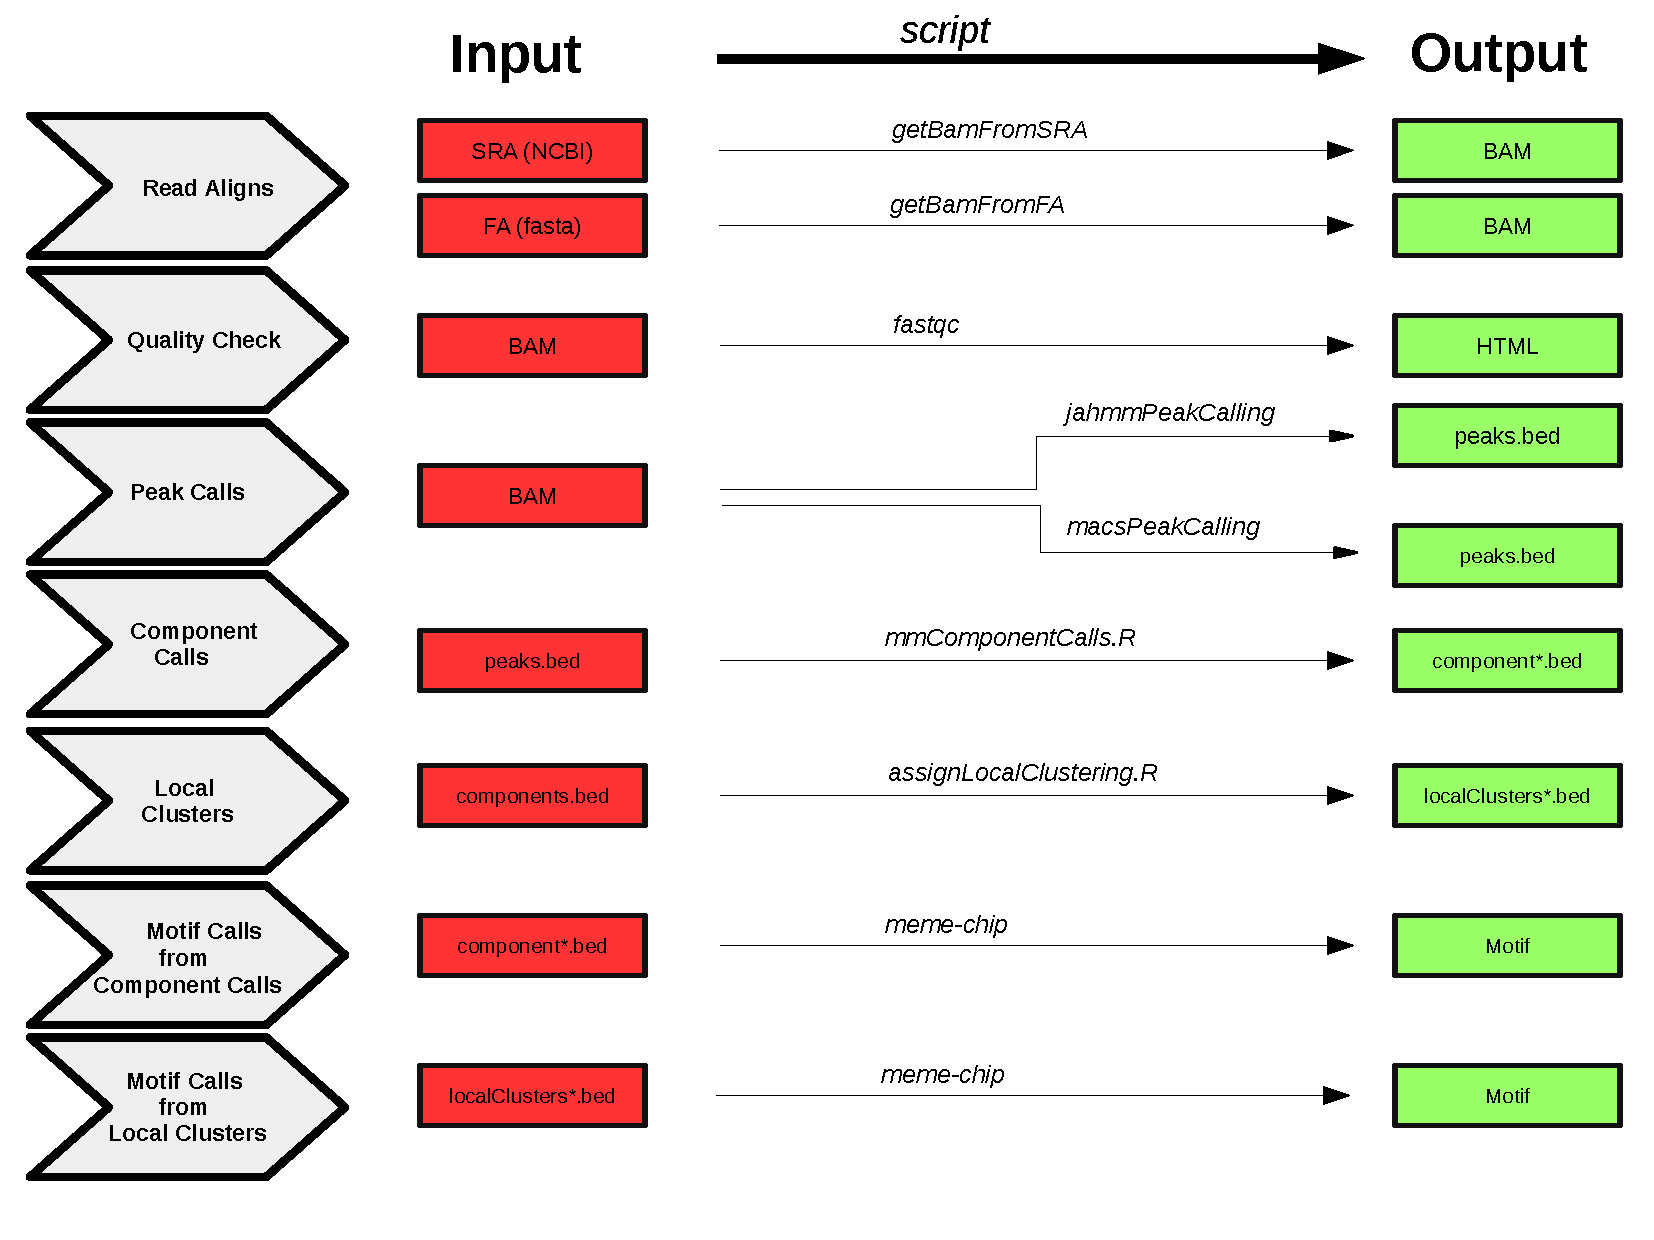
\includegraphics[width=0.7\textwidth]{/home/ricky/Rlim/ChromatinConformation/pipelineChart.pdf}} 
    \caption{Pipeline for Chromatin Conformation Prediction} 
\end{figure} 

\section{Implementation and Test}

\begin{verbatim}
# export PATH for scripts required 
PATH=$PATH:/home/ricky/Rlim/ChromatinConformation/Script;export PATH;
\end{verbatim}

\small{For more details information concerning the datasets please contact Nicolas Bertin for NF-$\kappa$B Zhao dataset and Cebp$\alpha$ with Samuel Collombet}



\subsection{Read Aligns}

\subsubsection{NF-$\kappa$B ChIPseq Transcription factor from Zhao, et al 2014}
The read dataset was obtained and aligned using bowtie by Nicolas Bertin (Fullwood Lab).
The dataset was in BAM format and sorted accordingly, as follows: 

\begin{verbatim}

ls *.bam | parallel -j 3 'samtools sort {} {.}.sorted' & 

\end{verbatim}

Only the sorted BAM files were stored.


\subsubsection{Cebp$\alpha$ ChIPseq in different cell lines from Samuel}
The read dataset was obtained and aligned by Samuel.
The dataset was downloaded from tblab-server at the following directory:

\verb |/DAS/TBlab/Samuel/raw/new/| 

The dataset was in BAM format and sorted accordingly, as follows: 

\begin{verbatim}
    ls *.bam | parallel -j 3 'samtools sort {} {.}.sorted' & 
\end{verbatim}

Only the sorted BAM files were stored.

\subsubsection{Cebp ChIPseq in from Porse}
The read dataset was obtained from NCBI with GEO GSE42321. 
The download link was stored in: 

\verb|/home/ricky/Rlim/ChromatinConformation/Input/SRA/Porse/sampleDownloadLinks.txt|

The dataset was stored in the following directory:

\verb|/home/ricky/Rlim/ChromatinConformation/Input/ReadAligns/Porse|            

\begin{verbatim}
Script/getBamFromSRA -c 2 -g /home/ricky/Rlim/Biotools/Genomes/mm10_bowtie2_index/bowtie2\ 
-a /home/ricky/Rlim/ChromatinConformation/Input/ReadAligns/Porse/annot.txt 
-i /home/ricky/Rlim/ChromatinConformation/Input/ReadAligns/Porse\
-o /home/ricky/Rlim/ChromatinConformation/Output/ReadAligns/Porse 2> Log/getBamFromSRA_Porse.txt 
\end{verbatim}

\subsubsection{Cebp ChIPseq in from Benner}
The read dataset was obtained from NCBI with GEO GSM537984. 
The download link was stored in:

\verb|/home/ricky/Rlim/ChromatinConformation/Input/FA/Benner/sampleDownloadLinks.txt|

The dataset was stored in the following directory:

\verb|/home/ricky/Rlim/ChromatinConformation/Input/ReadAligns/Benner|            

\begin{verbatim}
Script/getBamFromFA -c 2 -g /home/ricky/Rlim/Biotools/Genomes/mm10_bowtie2_index/bowtie2\
-a Input/ReadAligns/Benner/annot.txt -i Input/ReadAligns/Benner/ 
-o Output/ReadAligns/Benner/ 2> Log/getBamFromFA_Benner.txt
\end{verbatim}


\subsection{Quality Check}
\subsubsection{NF-$\kappa$B ChIPseq Transcription factor from Zhao, et al 2014}
\begin{verbatim}
ls Input/Bam/ZhaoB_etal.CellRep2014/*.bam |\ 
parallel -j 3 'fastqc -o Output/QC/ZhaoB_etal.CellRep2014/ {}' &\
\end{verbatim}

\subsubsection{Cebp$\alpha$ ChIPseq in different cell lines from Samuel}
\begin{verbatim}
ls Input/Bam/Samuel/*.bam |\ 
parallel -j 2 'fastqc -o Output/QC/Samuel {}' &\
\end{verbatim}

\subsubsection{Cebp ChIPseq in from Porse}
\begin{verbatim}
ls Input/QC/Porse/*.bam | parallel -j 2 'fastqc -o Output/QC/Porse/ {}'
\end{verbatim}

\subsubsection{Cebp ChIPseq in from Benner}
\begin{verbatim}
ls Input/QC/Benner/*.bam | parallel -j 2 'fastqc -o Output/QC/Benner/ {}'
\end{verbatim}

\subsection{Peak Calls}
We used \href{https://github.com/gui11aume/zerone/tree/master/doc}{jaHMM} for peak callings and macs2 peak caller.
jahmm library was downloaded and stored locally at 

\verb|/home/ricky/Rlim/ChromatinConformation/Library/jahmm|

\subsubsection{NF-$\kappa$B ChIPseq Transcription factor from Zhao, et al 2014}
\begin{verbatim}

Script/jahmmPeakCalling.sh -c 4 -g hg19 -r 300\ 
-i Input/PeakCalls/ZhaoB_etal.CellRep2014/\ 
-o Output/PeakCalls/Jahmm/ZhaoB_etal.CellRep2014/\ 
2> Log/jahmmPeakCall_ZhaoB.txt 


\end{verbatim}

\begin{verbatim}
   8599068 300bin-ZhaoB_etal.CellRep2014.ChIP-Seq_GM12878_cREL_Rep1.sorted_peaks.bed
   9382822 300bin-ZhaoB_etal.CellRep2014.ChIP-Seq_GM12878_cREL_Rep2.sorted_peaks.bed
   6144560 300bin-ZhaoB_etal.CellRep2014.ChIP-Seq_GM12878_p50_Rep1.sorted_peaks.bed
   5832975 300bin-ZhaoB_etal.CellRep2014.ChIP-Seq_GM12878_p50_Rep2.sorted_peaks.bed
   8622964 300bin-ZhaoB_etal.CellRep2014.ChIP-Seq_GM12878_p52_Rep1.sorted_peaks.bed
   8627622 300bin-ZhaoB_etal.CellRep2014.ChIP-Seq_GM12878_p52_Rep2.sorted_peaks.bed
   9384884 300bin-ZhaoB_etal.CellRep2014.ChIP-Seq_GM12878_p65_Rep1.sorted_peaks.bed
   9363618 300bin-ZhaoB_etal.CellRep2014.ChIP-Seq_GM12878_p65_Rep2.sorted_peaks.bed
   9398329 300bin-ZhaoB_etal.CellRep2014.ChIP-Seq_GM12878_RELB_Rep0.sorted_peaks.bed
\end{verbatim}

\begin{verbatim}

Script/macsPeakCalling.sh -c 4 -g hs\ 
-i Input/PeakCalls/ZhaoB_etal.CellRep2014/\
-o Output/PeakCalls/ZhaoB_etal.CellRep2014\ 
2> Log/macsPeakCall_Zhao.txt

\end{verbatim}

Number of peaks called by macs2 from Zhao datasets in majority are in millions. 
\begin{verbatim}
  1138227 ZhaoB_etal.CellRep2014.ChIP-Seq_GM12878_cREL_Rep1.sorted_summits_peaks.bed
  1045436 ZhaoB_etal.CellRep2014.ChIP-Seq_GM12878_cREL_Rep2.sorted_summits_peaks.bed
   445594 ZhaoB_etal.CellRep2014.ChIP-Seq_GM12878_p50_Rep1.sorted_summits_peaks.bed
   465586 ZhaoB_etal.CellRep2014.ChIP-Seq_GM12878_p50_Rep2.sorted_summits_peaks.bed
   984604 ZhaoB_etal.CellRep2014.ChIP-Seq_GM12878_p52_Rep1.sorted_summits_peaks.bed
   385493 ZhaoB_etal.CellRep2014.ChIP-Seq_GM12878_p52_Rep2.sorted_summits_peaks.bed
  3591979 ZhaoB_etal.CellRep2014.ChIP-Seq_GM12878_p65_Rep1.sorted_summits_peaks.bed
  3406538 ZhaoB_etal.CellRep2014.ChIP-Seq_GM12878_p65_Rep2.sorted_summits_peaks.bed
  3706260 ZhaoB_etal.CellRep2014.ChIP-Seq_GM12878_RELB_Rep0.sorted_summits_peaks.bed
\end{verbatim}

Number of peaks called by jahmm and macs from Zhao datasets are in millions.
As there are many peaks being called, the subsequent pipelines were not run for this dataset.

\subsubsection{Cebp$\alpa$ from Samuel}

Note that we used macs2 as the dataset from Samuel has not input and jahmm could call peaks without an input sample.

\begin{verbatim}

Script/macsPeakCalling.sh -c 4 -g hs\ 
-i Input/PeakCalls/Samuel/\ 
-o Output/PeakCalls/Macs/Samuel/\ 
2> Log/macsPeakCall_Samuel.txt

\end{verbatim}


\subsubsection{Cebp ChIPseq in from Porse}
 %mv Porse_Liver_ChIPseq_Input_mm10_rep0_q10rmdup.sorted.bam\
 %   Porse_Liver_ChIPseq_mm10_rep0_q10rmdup_Input.sorted.bam 
 %mv Porse_Liver_ChIPseq_CebpA_mm10_rep0_q10rmdup.sorted.bam\ 
 %   Porse_Liver_ChIPseq_mm10_rep0_q10rmdup_CebpA.sorted.bam 

\begin{verbatim}
Script/jahmmPeakCalling.sh -c 2 -g mm10 -r 300 -i Input/PeakCalls/Porse/\ 
 -o Output/PeakCalls/Jahmm/Porse/ 2> Log/jahmmPeakCall_Porse.txt
\end{verbatim}

\subsubsection{Cebp ChIPseq in from Benner}
%mv Benner_ThioMac_ChIPseq_CebpA_mm10_rep0_q10rmdup.sorted.bam\ 
%   Benner_ThioMac_ChIPseq_mm10_rep0_q10rmdup_CebpA.sorted.bam
%mv Benner_ThioMac_ChIPseq_Input_mm10_rep0_q10rmdup.sorted.bam\ 
%   Benner_ThioMac_ChIPseq_mm10_rep0_q10rmdup_Input.sorted.bam
\begin{verbatim}

Script/jahmmPeakCalling.sh -c 2 -g mm10 -r 300 -i Input/PeakCalls/Benner/\ 
-o Output/PeakCalls/Benner/ 2> Log/jahmmPeakCall_Benner.txt
\end{verbatim}


\subsection{Component Calls}

%\subsubsection{NF-$\kappa$B ChIPseq Transcription factor from Zhao, et al 2014}
%\begin{verbatim}
%Rscript Script/mmComponentCalls.R --model='GMM' --ncomp=3 --oneComp=TRUE\ 
%--input_dir='/home/ricky/Rlim/ChromatinConformation/Input/ComponentCalls/Jahmm/ZhaoB_etal.CellRep2014/'\
%--output_dir='/home/ricky/Rlim/ChromatinConformation/Output/ComponentCalls/Jahmm/ZhaoB_etal.CellRep2014/'\
%2> Log/mmComponentCall_ZhaoB.txt
%\end{verbatim}

\subsubsection{Cebp$\alpa$ from Samuel}
\begin{verbatim}

Script/mmComponentCalls.R --model='GMM' --ncomp=3 --oneComp=TRUE\ 
--input_dir='/home/ricky/Rlim/ChromatinConformation/Input/ComponentCalls/Macs/Samuel/'\ 
--output_dir='/home/ricky/Rlim/ChromatinConformation/Output/ComponentCalls/Macs/Samuel/'\ 
2> Log/mmComponentCall_Samuel.txt\

\end{verbatim}

\subsubsection{Cebp from Porse}
\begin{verbatim}
Rscript Script/mmComponentCalls.R --model='GMM' --ncomp=5 --oneComp=TRUE\ 
--input_dir='Input/ComponentCalls/Jahmm/Porse/'\
--output_dir='Output/ComponentCalls/Jahmm/Porse/' 2> Log/mmComponentCall_Porse.txt
\end{verbatim}

\subsubsection{Cebp from Benner}
\begin{verbatim}
Script/mmComponentCalls.R --model='GMM' --ncomp=3 --oneComp=TRUE\ 
--input_dir='Input/ComponentCalls/Jahmm/Benner/'\ 
--output_dir='Output/ComponentCalls/Jahmm/Benner/' 2> Log/mmComponentCall_Benner.txt
\end{verbatim}

\subsection{Local Clusters: Direct and Indirect}

\end{verbatim}

\subsubsection{Cebp$\alpa$ from Samuel}
\begin{verbatim}

Rscript Script/assignLocalClustering.R --distance=3000 --filter=TRUE\ 
--input_dir='/home/ricky/Rlim/ChromatinConformation/Input/LocalClusters/Macs/Samuel/'\ 
--output_dir='/home/ricky/Rlim/ChromatinConformation/Output/LocalClusters/Macs/Samuel/'\
2> Log/assignLocalCluster_Samuel.txt

\end{verbatim}

\subsubsection{Cebp from Porse}
\begin{verbatim}
Script/assignLocalClustering.R --distance=3000 --filter=TRUE\ 
--input_dir='/home/ricky/Rlim/ChromatinConformation/Input/LocalClusters/Jahmm/Porse/'\ 
--output_dir='/home/ricky/Rlim/ChromatinConformation/Output/LocalClusters/Jahmm/Porse/'
\end{verbatim}

\subsubsection{Cebp from Benner}
\begin{verbatim}
Script/assignLocalClustering.R --distance=3000 --filter=TRUE\ 
--input_dir='/home/ricky/Rlim/ChromatinConformation/Input/LocalClusters/Jahmm/Benner/'\ 
--output_dir='/home/ricky/Rlim/ChromatinConformation/Output/LocalClusters/Jahmm/Benner/'\ 
2> Log/assignLocalCluster_Benner.txt

\end{verbatim}

\subsection{Motif Calls from Component Calls}
\subsubsection{Cebp$\alpa$ from Samuel}

\begin{verbatim}
# extend bed peak summit from 1 bp resolution to 300 bp bin (150 bp in both strand directions)
# as samuel peaks were called using macs peak summit with 1 bp resolution
ls Input/MotifCalls/Macs/Samuel/ComponentCalls/*.bed |\ 
parallel -j 2 ``bedtools slop -i {}\ 
-g /home/ricky/Rlim/Biotools/Genomes/mm10/refGenome/mm10.genome\ -b 150 >{.}_150bp_extended.bed''

# bed to fasta
ls Input/MotifCalls/Macs/Samuel/ComponentCalls/*extended.bed |\ 
parallel -j 2 ``bedtools getfasta\ 
-fi /home/ricky/Rlim/Biotools/Genomes/mm10/refGenome/mm10.fa -bed {} -fo {.}.fa''

ls Input/MotifCalls/Macs/Samuel/ComponentCalls/*.fa |\ 
parallel -j 2 ``meme-chip\ 
-db /home/ricky/Rlim/Biotools/motif_databases/JASPAR_CORE_2014_vertebrates.meme\ 
-oc /home/ricky/Rlim/ChromatinConformation/Output/MotifCalls/Macs/Samuel/ComponentCalls/{/.}\ 
-index-name {/.} -meme-mod zoops -meme-minw 4 -meme-maxw 10 -meme-nmotifs 10 {}''

\end{verbatim}

\subsubsection{Cebp from Porse}
\begin{verbatim}
# convert the bed to fasta
ls Input/MotifCalls/Jahmm/Porse/ComponentCalls/*.bed |\ 
parallel -j 2 "bedtools getfasta\ 
-fi /home/ricky/Rlim/Biotools/Genomes/mm10/refGenome/mm10.fa -bed {} -fo {.}.fa"

# meme-chip
ls Input/MotifCalls/Jahmm/Porse/ComponentCalls/*.fa |\ 
parallel -j 2 "meme-chip -db ~/Rlim/Biotools/motif_databases/JASPAR_CORE_2014_vertebrates.meme\ 
-oc Output/MotifCalls/Jahmm/Porse/ComponentCalls{/.}\ 
-index-name {/.} -meme-mod zoops -meme-minw 4 -meme-maxw 10 -meme-nmotifs 10 {}"
\end{verbatim}

\subsubsection{Cebp from Benner}
\begin{verbatim}
# convert the bed to fasta
ls Input/MotifCalls/Jahmm/Benner/ComponentCalls/*.bed |\ 
parallel -j 2 "bedtools getfasta\ 
-fi /home/ricky/Rlim/Biotools/Genomes/mm10/refGenome/mm10.fa -bed {} -fo {.}.fa"

# meme-chip
ls Input/MotifCalls/Jahmm/Benner/ComponentCalls/*.fa |\ 
parallel -j 2 "meme-chip -db ~/Rlim/Biotools/motif_databases/JASPAR_CORE_2014_vertebrates.meme\ 
-oc Output/MotifCalls/Jahmm/Benner/ComponentCalls/{/.}\ 
-index-name {/.} -meme-mod zoops -meme-minw 4 -meme-maxw 10 -meme-nmotifs 10 {}"
\end{verbatim}

\subsection{Motif Calls from Local Clusters}
\subsubsection{Cebp$\alpa$ from Samuel}

\begin{verbatim}
# extend bed peak summit from 1 bp resolution to 300 bp bin (150 bp in both strand directions)
ls Input/MotifCalls/Macs/Samuel/LocalClusters/*.bed |\ 
parallel -j 2 ``bedtools slop -i {}\ 
-g /home/ricky/Rlim/Biotools/Genomes/mm10/refGenome/mm10.genome\ -b 150 >{.}_150bp_extended.bed''

# bed to fasta
ls Input/MotifCalls/Macs/Samuel/LocalClusters/*extended.bed |\ 
parallel -j 2 ``bedtools getfasta\ 
-fi /home/ricky/Rlim/Biotools/Genomes/mm10/refGenome/mm10.fa -bed {} -fo {.}.fa''

ls Input/MotifCalls/Macs/Samuel/LocalClusters/*.fa |\ 
parallel -j 2 ``meme-chip\ 
-db /home/ricky/Rlim/Biotools/motif_databases/JASPAR_CORE_2014_vertebrates.meme\ 
-oc /home/ricky/Rlim/ChromatinConformation/Output/MotifCalls/Macs/Samuel/LocalClusters/{/.}\ 
-index-name {/.} -meme-mod zoops -meme-minw 4 -meme-maxw 10 -meme-nmotifs 10 {}''

\end{verbatim}

\subsubsection{Cebp from Porse}
\begin{verbatim}
# convert the bed to fasta
ls Input/MotifCalls/Jahmm/Porse/LocalClusters/*.bed |\ 
parallel -j 2 "bedtools getfasta\ 
-fi /home/ricky/Rlim/Biotools/Genomes/mm10/refGenome/mm10.fa -bed {} -fo {.}.fa"

# meme-chip
ls Input/MotifCalls/Jahmm/Porse/LocalClusters/*.fa |\ 
parallel -j 2 "meme-chip -db ~/Rlim/Biotools/motif_databases/JASPAR_CORE_2014_vertebrates.meme\ 
-oc Output/MotifCalls/Jahmm/Porse/LocalClusters{/.}\ 
-index-name {/.} -meme-mod zoops -meme-minw 4 -meme-maxw 10 -meme-nmotifs 10 {}"
\end{verbatim}

\subsubsection{Cebp from Benner}
\begin{verbatim}
# convert the bed to fasta
ls Input/MotifCalls/Jahmm/Benner/LocalClusters/*.bed |\ 
parallel -j 2 "bedtools getfasta\ 
-fi /home/ricky/Rlim/Biotools/Genomes/mm10/refGenome/mm10.fa -bed {} -fo {.}.fa"

# meme-chip
ls Input/MotifCalls/Jahmm/Benner/LocalClusters/*.fa |\ 
parallel -j 2 "meme-chip -db ~/Rlim/Biotools/motif_databases/JASPAR_CORE_2014_vertebrates.meme\ 
-oc Output/MotifCalls/Jahmm/Benner/LocalClusters/{/.}\ 
-index-name {/.} -meme-mod zoops -meme-minw 4 -meme-maxw 10 -meme-nmotifs 10 {}"
\end{verbatim}


\begin{verbatim}
  Filename: chromatinConformation.Rnw
  Working directory: /home/ricky/Rlim/ChromatinConformation 
\end{verbatim}

\section{Metainfo}
\begin{knitrout}
\definecolor{shadecolor}{rgb}{0.969, 0.969, 0.969}\color{fgcolor}\begin{kframe}
\begin{alltt}
\hlkwd{sessionInfo}\hlstd{()}
\end{alltt}
\begin{verbatim}
## R version 3.2.1 (2015-06-18)
## Platform: x86_64-pc-linux-gnu (64-bit)
## Running under: Ubuntu 14.04.1 LTS
## 
## locale:
##  [1] LC_CTYPE=en_SG.UTF-8       LC_NUMERIC=C              
##  [3] LC_TIME=en_SG.UTF-8        LC_COLLATE=en_SG.UTF-8    
##  [5] LC_MONETARY=en_SG.UTF-8    LC_MESSAGES=en_SG.UTF-8   
##  [7] LC_PAPER=en_SG.UTF-8       LC_NAME=C                 
##  [9] LC_ADDRESS=C               LC_TELEPHONE=C            
## [11] LC_MEASUREMENT=en_SG.UTF-8 LC_IDENTIFICATION=C       
## 
## attached base packages:
## [1] stats     graphics  grDevices utils     datasets  methods   base     
## 
## other attached packages:
## [1] knitr_1.10.5
## 
## loaded via a namespace (and not attached):
## [1] magrittr_1.5  formatR_1.2   tools_3.2.1   stringi_0.5-2 highr_0.5    
## [6] digest_0.6.8  stringr_1.0.0 evaluate_0.7
\end{verbatim}
\end{kframe}
\end{knitrout}




\end{document}
